\documentclass[12pt]{article}
\usepackage{graphicx}
\pagestyle{empty}
\usepackage[urlcolor=blue,colorlinks=true]{hyperref}

\setlength{\parindent}{0mm}
\setlength{\parskip}{2mm}

\setlength{\oddsidemargin}{0mm}
\setlength{\evensidemargin}{0mm}
\setlength{\topmargin}{-12mm}
\setlength{\textheight}{240mm}
\setlength{\textwidth}{158mm}

\title{GF Resource Grammar Summer School}
\author{Gothenburg, 17-28 August 2009}
\begin{document}

\begin{center}
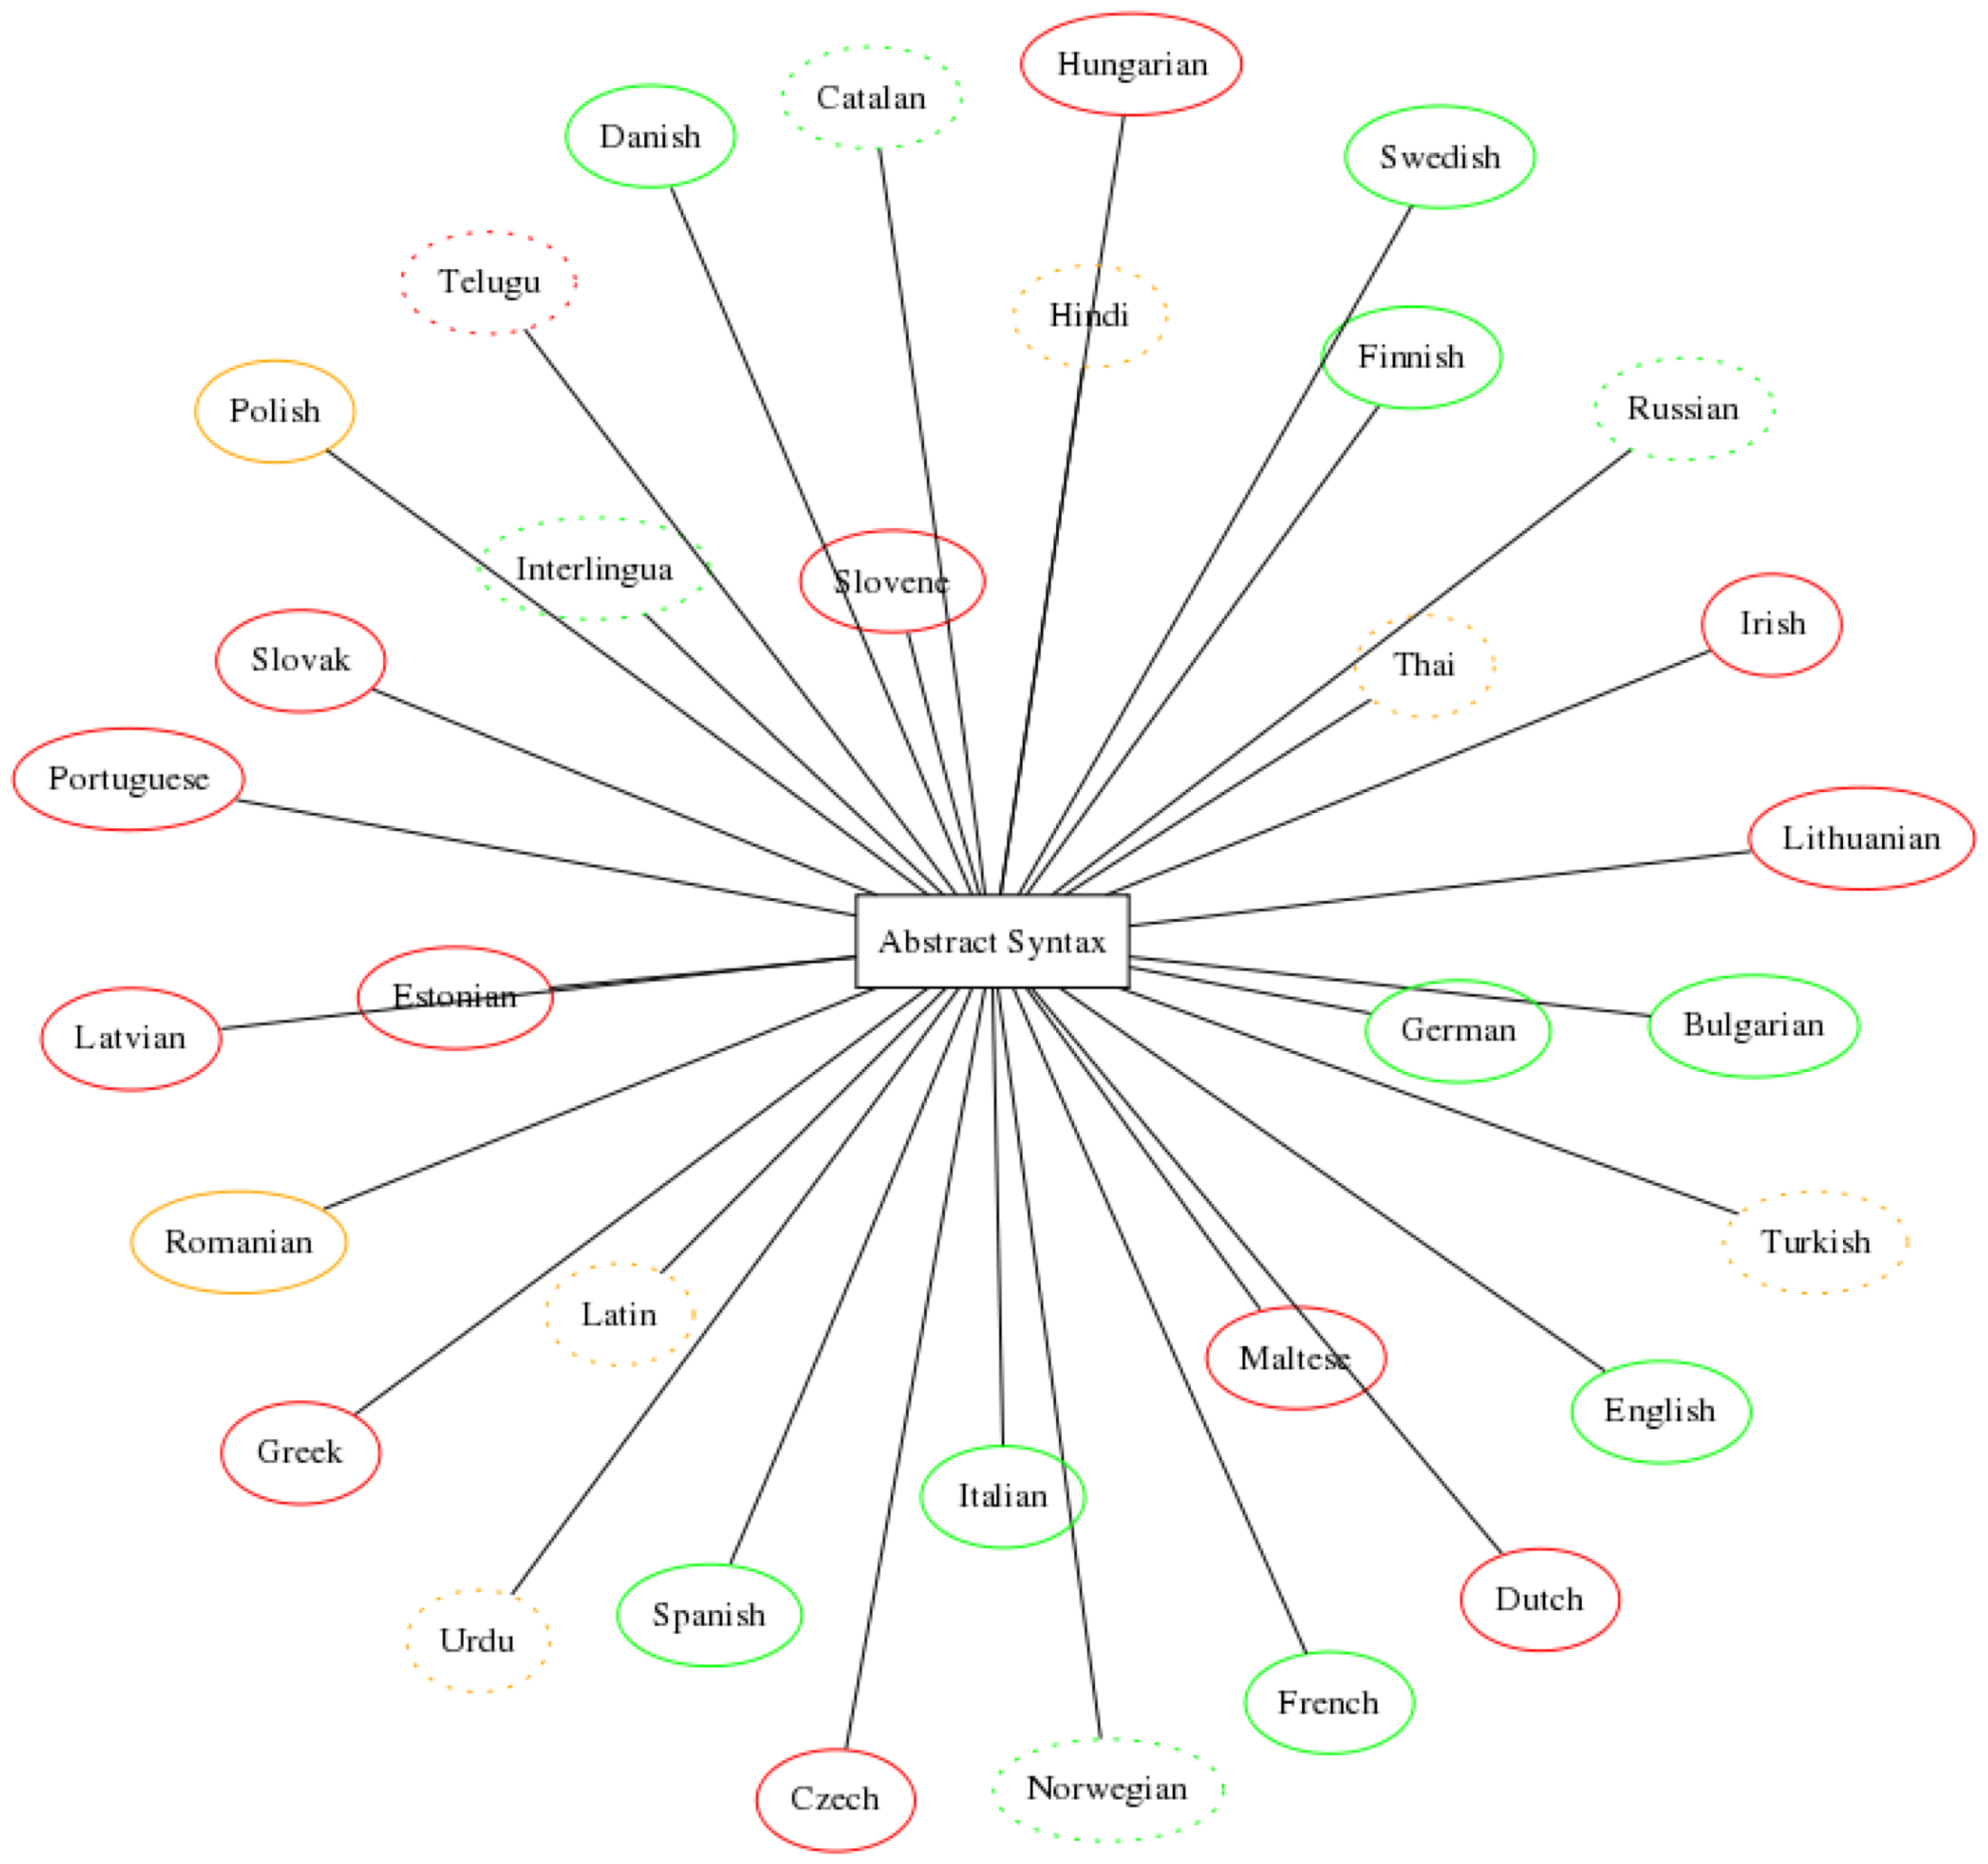
\includegraphics{summer-langs.png}

\vspace{6mm}

{\Large\bf GF Resource Grammar Summer School}

\vspace{2mm}

Gothenburg, 17-28 August 2009

\vspace{6mm}

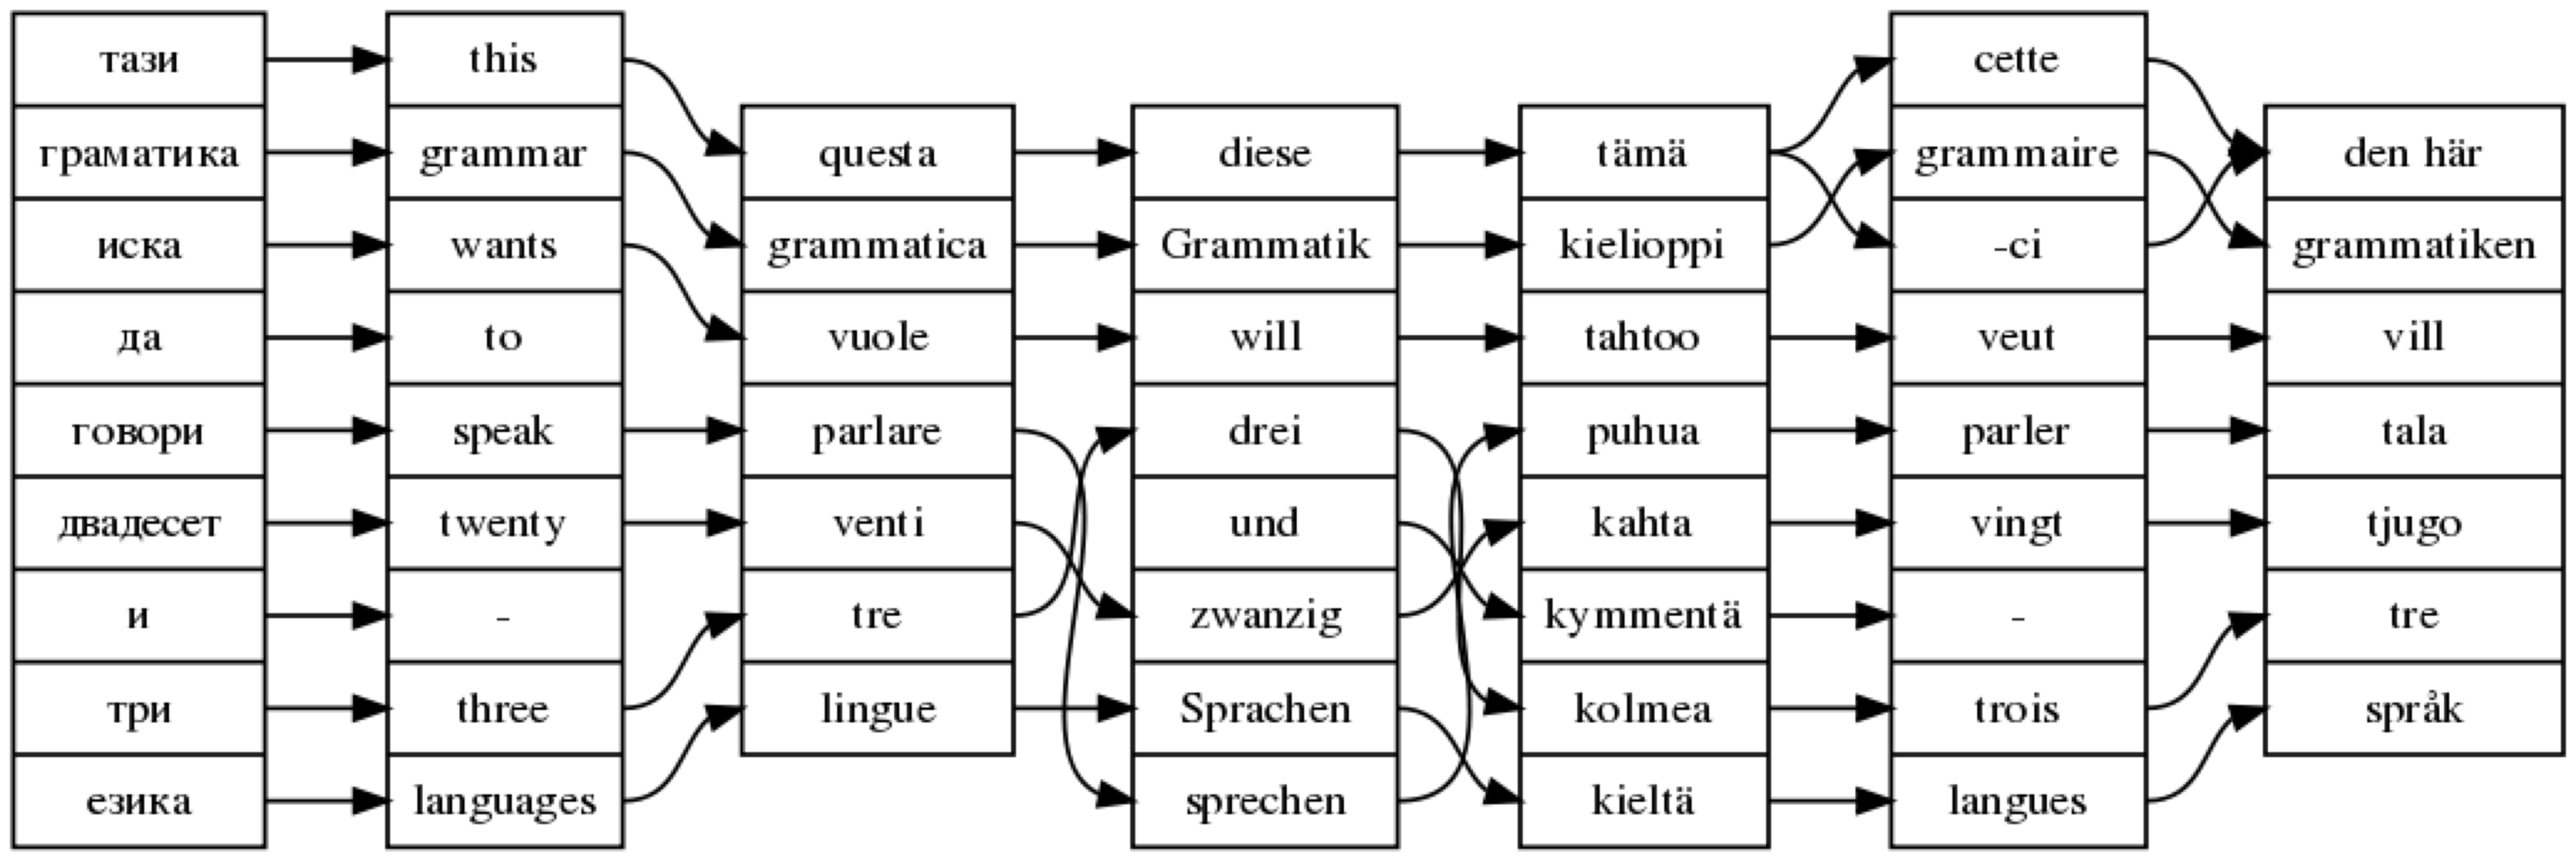
\includegraphics{summer-align.png}
\end{center}

\newpage

\begin{itemize}
\item Do you like programming challenges? 
\item Are you interested in how your language really works? 
\item Would you like to try and build a computational grammar for your language, 
  and make it available as a part of an international open-source 
  programming effort? 
\end{itemize}

Then you should consider attending the GF Resource Grammar Summer School 
in Gothenburg on 17-28 August 2009.

The GF Resource Grammar Library is an open-source computational grammar 
resource that currently covers 12 languages. It has been created in 
a collaborative effort using the GF (Grammatical Framework) grammar formalism.
The Summer School aims to boost the extension of the library to new languages.

Particularly in focus are the missing 12 of the 23 official languages of the 
European Union: \textit{Czech, Dutch, 
Estonian, Greek, Hungarian, Irish, Latvian, Lithuanian,
Maltese, Portuguese, Slovak, and Slovenian}. There is also more work to
be done on Polish and Romanian.
Any other languages chosen by the participants are also welcome.
Good knowledge of the language is essential, but you don't need to be a 
native speaker.

The linguistic coverage of the library includes the inflectional morphology
and basic syntax of each language. It can be used for parsing,
generation, translation, multilingual web pages, 
speech recognition, dialogue systems, language teaching, morphological
analysis, software localization, and lots of other things. 
Grammars written in GF can be converted to many different formats. 
The library is licensed under LGPL.

In the summer school, each language will be implemented by one or two students
working together. A morphology implementation will be credited
as a Chalmers University
course worth 7.5 ETCS points; adding a syntax implementation
will be worth more. The estimated total work load is 1-2 months for the
morphology, and 3-6 months for the whole grammar.

Participation in the summer school is free. 
Registration is via the courses's Google group,

\begin{verbatim}
 http://groups.google.com/group/gf-resource-school-2009/
\end{verbatim}
The registration deadline is 15 June 2009. An on-line course on GF (recommended,
but not compulsory) starts on 20 April.

Some travel grants will be available. They are distributed on the basis of a
GF programming contest in May.

For more information, see the Google Group and the Summer School web page,

\begin{verbatim}
 http://digitalgrammars.com/gf/summerschool.html
\end{verbatim}

% LaTeX2e code generated by txt2tags 2.4 (http://txt2tags.sf.net)
% cmdline: txt2tags summerschool-folder.txt
\end{document}
